\chapter{Sistemas ABC On-the-fly}\label{ch:ABC_OnTheFly}

La tendencia es el despliegue de sistemas \GLS{ABC} \gls{OnTheFly} \cite{raghavendra2013robust}. Este enfoque es mucho más cómodo para el viajero porque todo el proceso se puede hacer mientras el pasajero está caminando. Esto significa que los algoritmos de verificación facial tienen que funcionar tan pronto como una cara es detectada, sin requerir una pose estática o la colaboración del usuario. Gran parte de los estudios sobre sistemas \GLS{ABC} \gls{OnTheFly} se centran en la verificación facial y no se ha encontrado ninguno que analice la problemática específica de los \GLS{PAD} para este tipo de sistemas.

En este capitulo se presenta un sistema \GLS{PAD} para para sistemas \GLS{ABC} \gls{OnTheFly} (\gls{FlyPAD}) que implementa un conjunto de técnicas dinámicas para detectar múltiples tipos de ataques de presentación en biometría facial (fotos impresas, máscaras de papel, máscaras de papel sin ojos, vídeos en pantalla y máscaras $3$D), mientras el viajero cruza el sistema, sin necesidad de detenerse frente a las cámaras. 

Para ilustrar el comportamiento del sistema y medir su rendimiento se han llevado a cabo experimentos en un entorno controlado (es decir, en un laboratorio) y experimentos un escenario fronterizo real, comparando las capacidades del sistema \GLS{PAD} en situaciones estáticas y dinámicas.

El capitulo se organiza de la siguiente manera: En la Sección \ref{sec:SistemaFlayPAD} se presentan los fundamentos del sistema propuesto y en la Sección \ref{sec:ArquitecturaFlayPAD} se detalla su arquitectura, mientras que la sección \ref{sec:ExpermentosFlayPAD} aborda los diferentes experimentos realizado y los resultados obtenidos. Y por último, la Sección \ref{sec:ConclusuionesFlayPAD} concluye y proporciona las futuras directrices.

%%%%%%%%%%%%%% SISTEMA FlyPAD %%%%%%%%
\section{Sistema FlyPAD}\label{sec:SistemaFlayPAD}

\begin{figure}[t!]
    \centering
    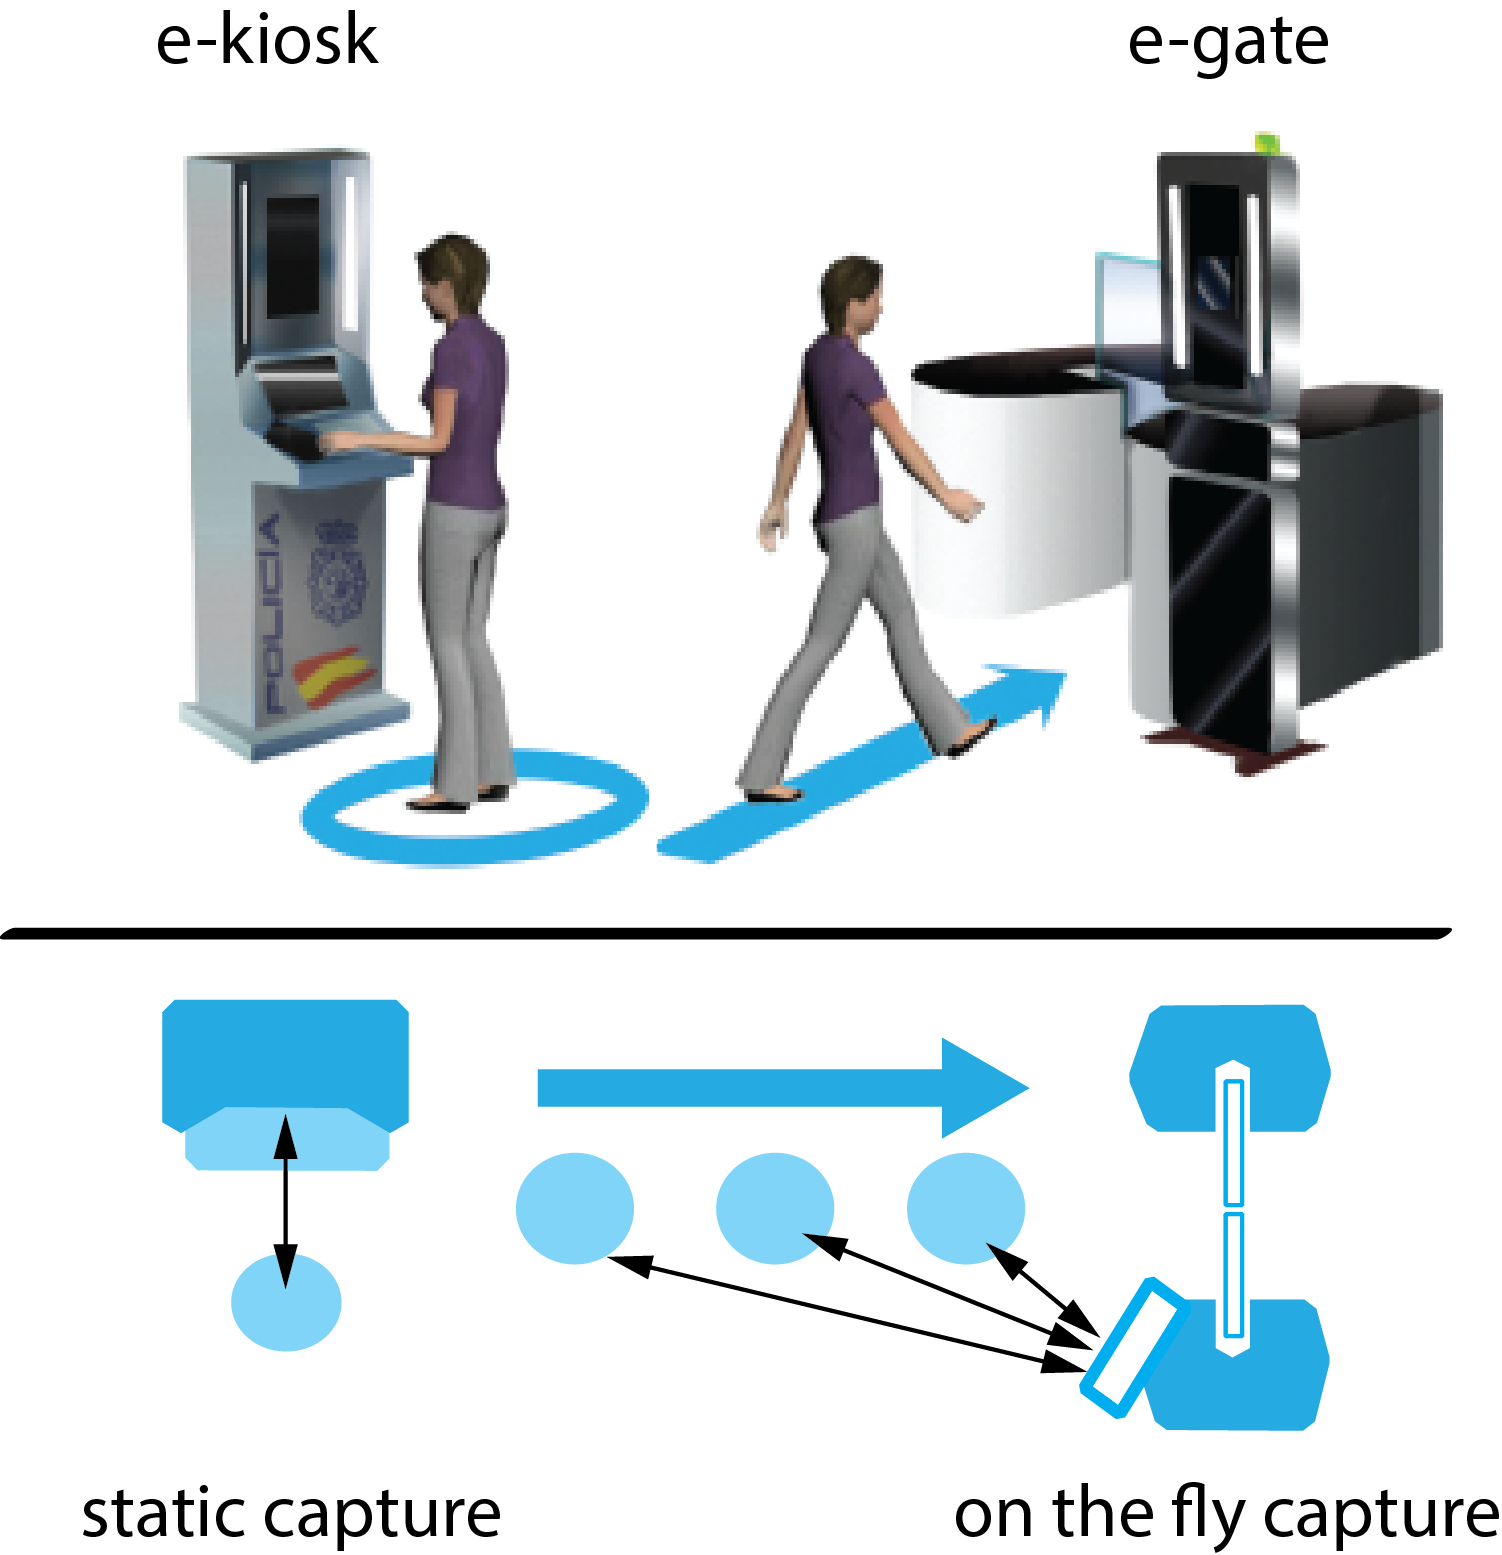
\includegraphics[width=.5\textwidth]{ch-sistemasABC/images/ch-onthefly/GraficaKioskGate.png}
    \caption{Vista esquemática superior de la puerta electrónica, con el quiosco de registro (izquierda) y la puerta electrónica (derecha). Abajo: Adquisición de la cara para la captura estática y dinámica.}
    \label{fig:staticvsdynamic}
\end{figure}

\gls{FlyPAD} es un sistema de detección de ataques de presentación diseñado para sistemas \textit{<<Segregated Two Step>>} \GLS{ABC} (ver topologías \GLS{ABC} en Sección \ref{subsec:Topologias}) donde existe una etapa de registro (en un dispositivo \gls{e-kiosk} para los experimentos), previa al cruce real de la frontera en un \gls{e-gate}. La captura en el registro se realiza de forma estática mientras que la en el cruce es dinámica.

Aunque la captura la \gls{e-gate} sea \gls{OnTheFly}, el cruce de fronteras deber realizarse de forma individual y los viajeros deben haber sido previamente registrados. Es necesario que cada viajero haya presentado su documentación de viaje y el sistema haya capturado su información biométrica antes proceder al cruce.

Aunque \gls{FlyPAD} tiene el \GLS{PAD} dinámico como su principal objetivo, el sistema también puede realizar su tarea con una configuración estática (ver Fig. \ref{fig:staticvsdynamic}). Por eso el sistema ha sido puesto a prueba tanto en la etapa registro como en el cruce y se ha instalando en el \gls{e-kiosk} y en el \gls{e-gate}.


%%%%%%%%%%%%%% ARQUITECTURA FlyPAD %%%%%%%%
\section{Arquitectura del sistema FlyPAD}\label{sec:ArquitecturaFlayPAD}

\begin{figure}[t!]
    \centering
    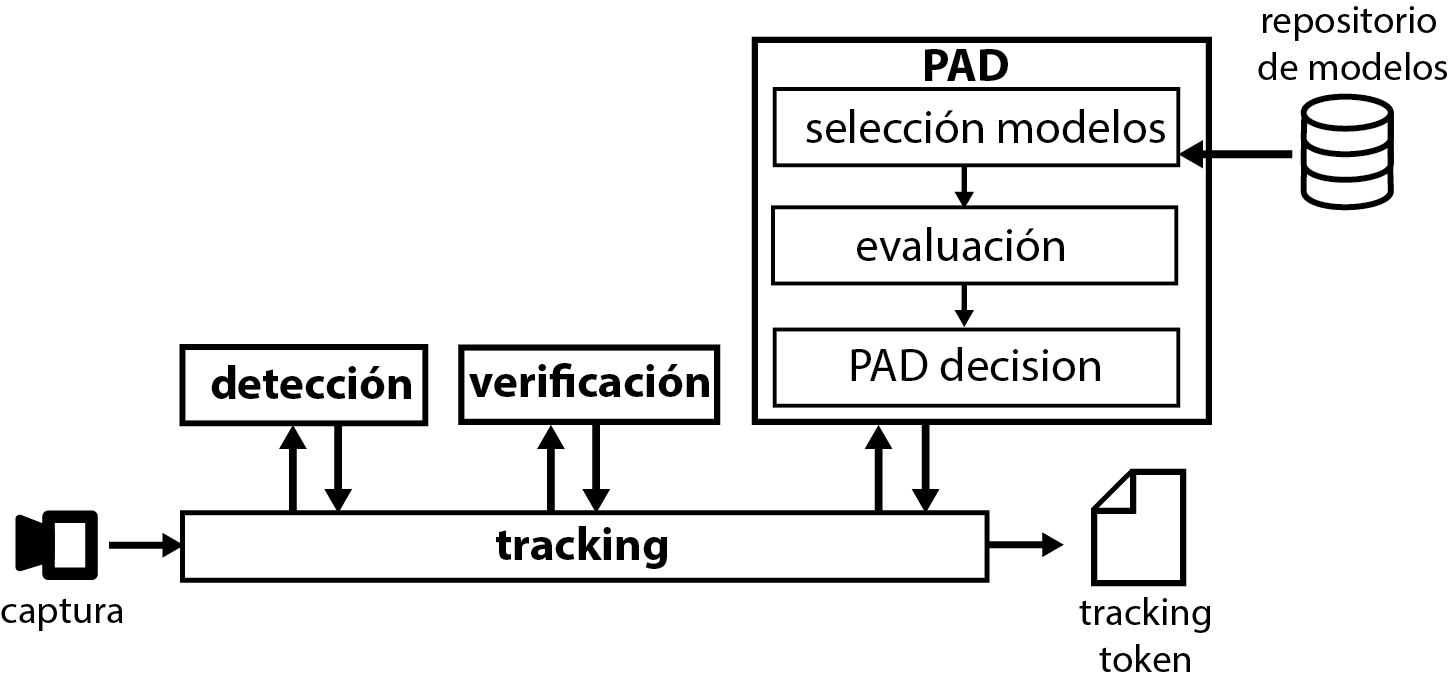
\includegraphics[width=.8\textwidth]{ch-sistemasABC/images/ch-onthefly/GRAFICA-PROCESO.png}
    \caption{Arquitectura del sistemas \gls{FlyPAD}.}
    \label{fig:architecture}
\end{figure}

Parámetros como la iluminación, la pose o la distancia a la cámara están extremadamente controlados en los sistemas \GLS{PAD} estáticos, pero son muy difíciles de controlar en escenarios dinámicos. Para ello se requiere de el desarrollo de técnicas capaces de resolver estos problemas que en el caso de \gls{FlyPAD} han sido incluidas en los diferentes componentes de la arquitectura del sistema.

La arquitectura de \gls{FlyPAD} se compone de cuatro módulos: \textit{Tracking}, Detección, Verificación y \GLS{PAD}. Y además hay que considerar tres componentes esenciales: el dispositivo de captura, el repositorio de modelos y el \textit{Tracking Token} (ver Fig. \ref{fig:architecture}).

El módulo de \textit{tracking} es el elemento subyacente y supervisa el movimiento de los viajeros durante su aproximación a la puerta electrónica: localiza a los viajeros mediante el módulo de detección, valida su identidad mediante el de verificación y detecta los posibles ataques con el módulo \GLS{PAD}.

%%%%%%%% MODULO DE TRACKING
\subsection{Módulo de Tracking}

\begin{figure}[t!]
    \centering
    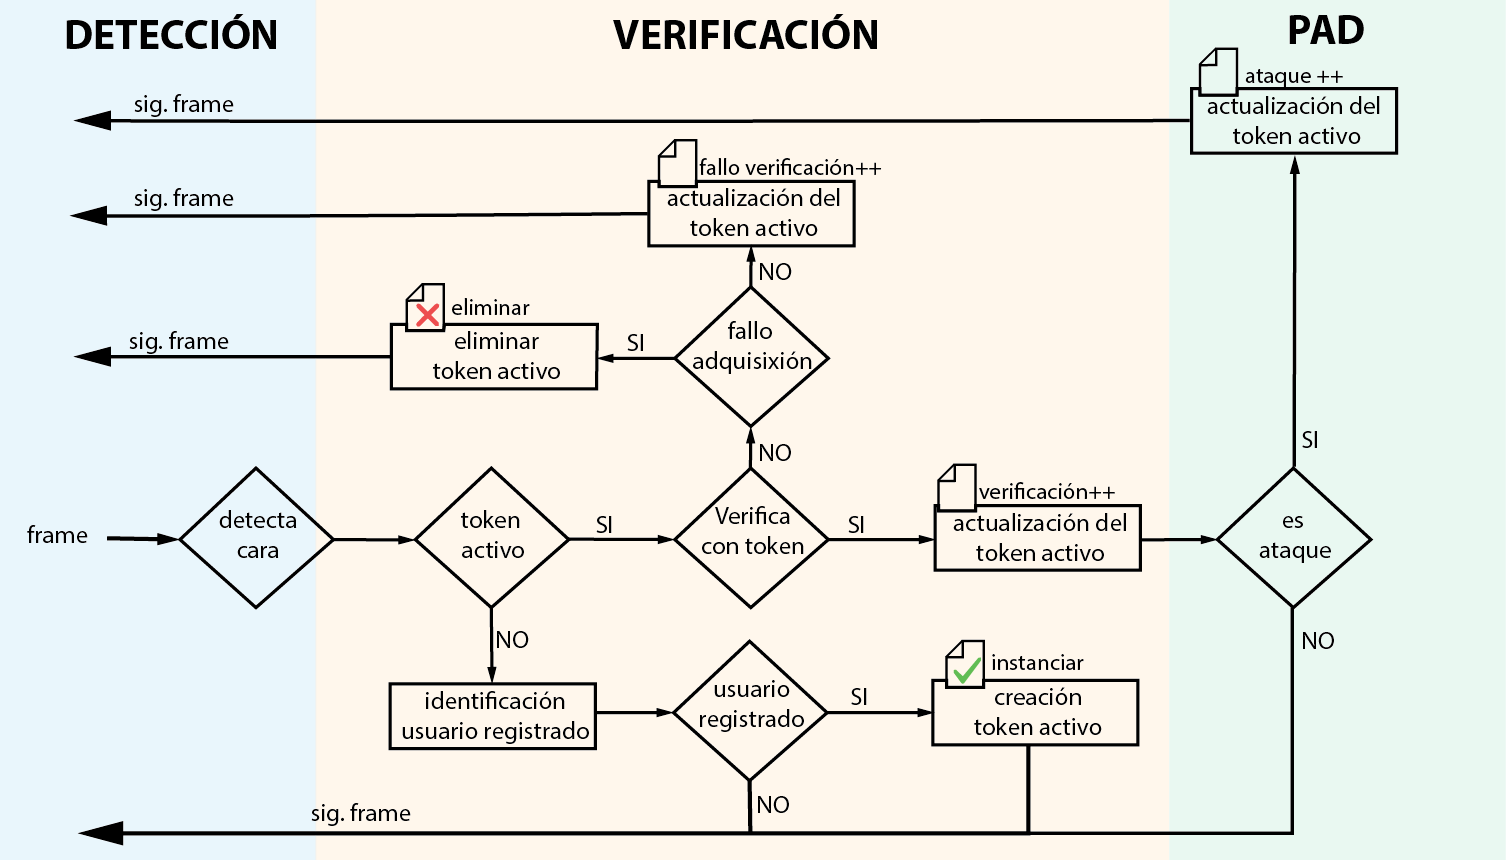
\includegraphics[width=1\textwidth]{ch-sistemasABC/images/ch-onthefly/DIAGRAMA_FLUJO_FLYPAD.png}
    \caption{Diagrama del proceso del módulo de \textit{Tracking} de \gls{FlyPAD}.}
    \label{fig:diagramaTracking}
\end{figure}

El módulo de \textit{tracking} funciona en consonancia con el resto de módulos con los que intercambia información. De esta forma, recibe $25$ fps (fotogramas por segundo)  de $1,920\times1,080$ píxeles del dispositivo de captura. Sólo {uno de cada cinco fotogramas capturados es procesado} por el módulo de detección. Si se detecta una cara, el módulo de detección devuelve la región en la que se encontraba la cara y estima la distancia al dispositivo de captura. Cada cara es evaluada por el módulo de verificación para identificar al viajero y por el módulo \GLS{PAD} para detectar posibles ataques (ver Fig. \ref{fig:diagramaTracking}). 

Cuando se localiza por primera vez la cara de alguno de los viajeros registrados el módulo de \textit{tracking} instancia un \textit{Tracking Token} asociado a la identidad de este viajero. Este \textit{Token} estará activo hasta que el viajero cruce la frontera. Cada vez que se detecte una nueva cara, ésta se compara con el \textit{Token} activo para decidir si corresponde a la misma identidad. En caso de verificación positiva, se actualiza la información del \textit{Token} incrementando el número de coincidencias de la identidad. Si durante cinco\footnote{El número de verificaciones negativas consecutivas ha sido estimado mediante en base a la experiencia adquirida con las pruebas realizadas.} verificación negativas consecutivas con el \textit{Token} activo, el modulo de \textit{Tracking} considerará que se ha producido un fallo de adquisición y el \textit{Token} actual será descartado.

El \textit{Token} además de la información de identidad también almacena información del \textit{tracking} del viejo, como los resultados del módulo de verificación o los resultados del módulo \GLS{PAD}. Cuando los viajeros se encuentran finalmente frente al \gls{e-gate}, la información del \textit{Token} se utiliza para decidir si pueden cruzar o no la frontera. Si el \textit{Token} contiene más de una cierta cantidad de pasos de \textit{tracking} autenticados (es decir, presentaciones \gls{bona-fide} \cite{ramachandra2017presentation}), entonces el sistema permite el cruce del viajero. De lo contrario, si el módulo \GLS{PAD} detecta marcos de seguimiento anómalos, el sistema considera al viajero como un atacante. En este caso se requiere una verificación manual por parte de los agentes de seguridad.

%%%%%%%% MODULO DE DETECCION
\subsection{Módulo de detección}

Este módulo se encarga de localizar caras en cada uno de los fotogramas recibidos, mediante el algoritmo \textit{Viola-Jones} \cite{viola2004robust} y calcula una estimación de la distancia del viajero al \gls{e-gate}, considerando la resolución de la cámara y el tamaño de la región detectada.

Con el fin de optimizar el sistema. se consideran tres rangos de distancias como los establecidos para \Gls{FRAV-OnTheFly} y para \Gls{FRAV-ABC-OnTheFly} (ver Sección \ref{sec:BBDD-OnTheFly}): El primer rango, cuando la distancia al dispositivo de captura es superior a $2$ m, el segundo, para distancias mayores de $1$ m y menores de $2$ m. Y el tercero con distancias menores de $1$ m al dispositivo de captura. 

Para establecer el rango de distancias se considera el tamaño de las regiones detectadas respecto a la resolución de la cámara. Las regiones con menos de $50\times50$ píxeles son descartadas, ya que están demasiado lejos y son muy pequeñas para ser verificadas. Las regiones entre $50\times50$ y $150\times150$ píxeles se consideran del primer rango. Las regiones entre $150 \times 150$ y $250\times250$ píxeles del segundo rango, y las regiones mayores de $250\times250$ píxeles del tercer rango (ver Tabla \ref{tab:facesranges_FRAV_OnTheFly}. 

%%%%%%%% MODULO DE VERIFCACION
\subsection{Módulo de verificación}

Este módulo debe verificar la identidad de la cara detectada. Si existe un \textit{token} activo, es decir, si se está realizando el \textit{tracking} de una determinada identidad, la verificación (($1$:$1$)) se realiza entre la cara detectada y la cara registrada correspondiente a dicho \textit{token}. Mientras que si aun no se está realizando un \textit{tracking}, es necesario un proceso de identificación ($1$:$n$) entre los usuarios registrados. para localizar la identidad del viajero y crear un nuevo \textit{Tracking Token} con ella.

Tanto la identificación como la verificación se realizan con un \textit{software} comercial de reconocimiento facial \textit{Cognitec} \cite{cognitec2019url}, especializado en documentos de viaje y cuyo algoritmo está en el \textit{top-ten} del \textit{ranking} de rendimiento en la prueba \GLS{NIST} FRVT $1$:$1$ (\textit{Face Recognition Vendor Test}) con imágenes de visado \cite{chen2016unconstrained}.

%%%%%%%% MODULO DE VERIFCACION
\subsection{Módulo PAD}

El módulo \GLS{PAD} evalúa si la cara detectada es un ataque o una presentación \textit{\gls{bona-fide}}. Esta tarea de detección se realiza en tres etapas (ver Fig. \ref{fig:architecture}): La selección del modelos, la evaluación y la toma de decisión.

\medskip
\textbf{Selección de modelos} % SELECCION DE MODELOS

En la primera etapa, se seleccionan del reposición de modelos, los clasificadores apropiados para evaluar la captura realizara. Se seleccionan cinco clasificadores (uno por cada tipo de ataque) atendiendo a la distancia detección.

\medskip
\textbf{Evaluación} % EVALAUCION

La región con la cara capturada se escala a una resolución de $100\times100$ píxeles y se calcula el histograma \GLS{LBP} \cite{ojala1996comparative}, usado como vector de características por los clasificadores. De cada clasificador se obtiene un \textit{score} con la probabilidad de que la cara sea el ataque que cada uno de ellos es capaz de detectar.  

\medskip
\textbf{Toma de decisión} % DECISION

Calculando la media de los \textit{scores} obtenidos de cada clasificador se obtiene la probabilidad conjunta de que la cara detectada, sea alguno de ataques contemplado. 
\medskip

Determinar finamente si la cara es o no un ataque requiere la selección de un umbral para la probabilidad media. El umbral depende del valor de confianza deseado (es decir, ponderar entre seguridad y conveniencia: ¿cuántos ataques puede aceptar el sistema? o ¿cuántas alarmas innecesarias generará?). En el caso de los sistemas \GLS{ABC}, \Gls{frontex} establece unos criterios para fijar este umbral \cite{FRONTEX2016OpeReport}.


%%%%%%%% REPOSITORIO DE MODELOS
\subsection{Repositorio de modelos} 

El repositorio de modelos almacena los diferentes modelos de aprendizaje entrenados para el sistema. Cada modelo consiste en clasificador \GLS{SVM} \cite{ma2014support} bi-clase lineal (ataque o \textit{\gls{bona-fide}}) similar a los descritos en \cite{chingovska2012effectiveness}.

Los clasificadores se organizan en tres conjuntos ateniendo a los rangos distancias (Rango-1, Rango-2 o Rango-3), con cinco clasificadores por conjunto, uno por cada \GLS{PAI} considerado (foto, máscara de papel, máscara de papel sin ojos, vídeo o máscara $3$D). Esta organización está motivada por el hecho de que los clasificadores especializados presentan mejores resultados que un único clasificador entrenado con todos los ataques y para todas las distancias \cite{goto2011pedestrian}). Y además, resulta flexible, permitiendo que se añadan nuevos \GLS{PAI} sin necesidad de volver a entrenar todos los clasificadores o alterar la arquitectura del sistema.

Todos los \GLSpl{SVM} han sido entrenados utilizando el $70$\% de los vídeos almacenados en la base de datos \Gls{FRAV-OnTheFly} (Sección \ref{subsec:BBDD-FRAV-OnTheFly}).

%%%%%%%%%%%%%% EPERIMENTOS Y RESULTADOS %%%%%%%%
\section{Experimentos y resultados}\label{sec:ExpermentosFlayPAD}

Esta sección presenta el conjunto de experimentos realizados para ilustrar la viabilidad de \gls{FlyPAD}. Se han realizado pruebas en dos escenarios, con los que se han construido dos bases de datos: \Gls{FRAV-OnTheFly} que contiene vídeos obtenidos en un ambiente controlado, simulando, en un laboratorio el comportamiento de los viajeros que cruzan un sistema \GLS{ABC} \gls{OnTheFly}. Y \Gls{FRAV-ABC-OnTheFly} con vídeos de viajeros en un cruce de frontera real (Para ver una descripción más detallada de las base de datos ver las secciones \ref{subsec:BBDD-FRAV-ABC-OnTheFly} y \ref{subsec:BBDD-FRAV-ABC-OnTheFly}).

La precisión del sistema depende del número de \textit{frames} consecutivos detectados con una misma identidad necesarios para considerar un \textit{tracking} como \textit{tracking} válido (\textit{consecutive frames}, \GLS{CF}), y del  porcentaje de \textit{bona-fide} \textit{frames} \GLS{BFF} necesarios para etiquetar el \textit{tracking} válido como \textit{tracking \gls{bona-fide}}. Por ejemplo, en Fig. \ref{fig:ranges-APCER-BPCER-RESULT_OnTheFly} (b), el sistema obtiene una precisión del $89,5$\% cuando se establece que un \textit{tracking} valido debe tener como mínimo $15$ \GLS{CF} y un porcentaje del $10$\% de \GLS{BFF}. Sin embargo, la precisión es sólo del $60,2$\%, cuando se requieren  $60$ \GLS{CF} y un $30$\% de \GLS{BFF}.

\begin{itemize}
    \item 
    \textbf{\GLS{CF} (\textit{Consecutive Frames})}: Número de \textit{frames} consecutivos en los que se ha detectado una identidad para considera un \text{tracking} como \textit{tracking} valido.
    \item 
    \textbf{\GLS{BFF} (\textit{\Gls{bona-fide} Frames})}: Porcentaje de \textit{frames} que el módulo \gls{PAD} considera \textit{bona-fide}, en un \textit{tracking valido}, para sea considerado un \textit{tracking bona-fide}.
\end{itemize}

A continuación se presentan los resultados obtenidos con los vídeos para test de \Gls{FRAV-OnTheFly}, y con todos los vídeos de \Gls{FRAV-ABC-OnTheFly}. En ambas situaciones, se incluyen los resultados con y sin el módulo de \textit{tracking} activado (es decir, situaciones dinámicas y estáticas).

\subsection{Resultados del escenario de línea de base controlada}%% EN LABORATORIO

\begin{figure}[t!]
    \centering
    \begin{subfigure}{.45\textwidth}
        \centering
        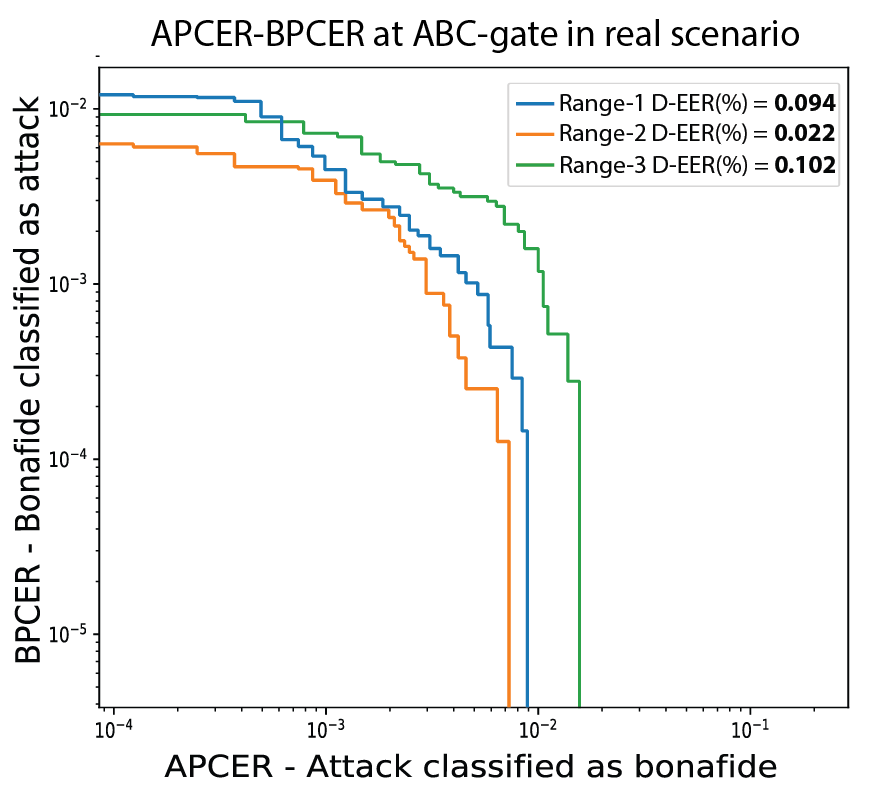
\includegraphics[width=1\linewidth]{ch-sistemasABC/images/ch-onthefly/APCER-BPCER-AT-DEVICE_b.png}
        \caption{Resultados del modulo \GLS{PAD} por rango.}
        \label{fig:pad-result-DATABASE}
    \end{subfigure}
    \begin{subfigure}{.45\textwidth}
        \centering
        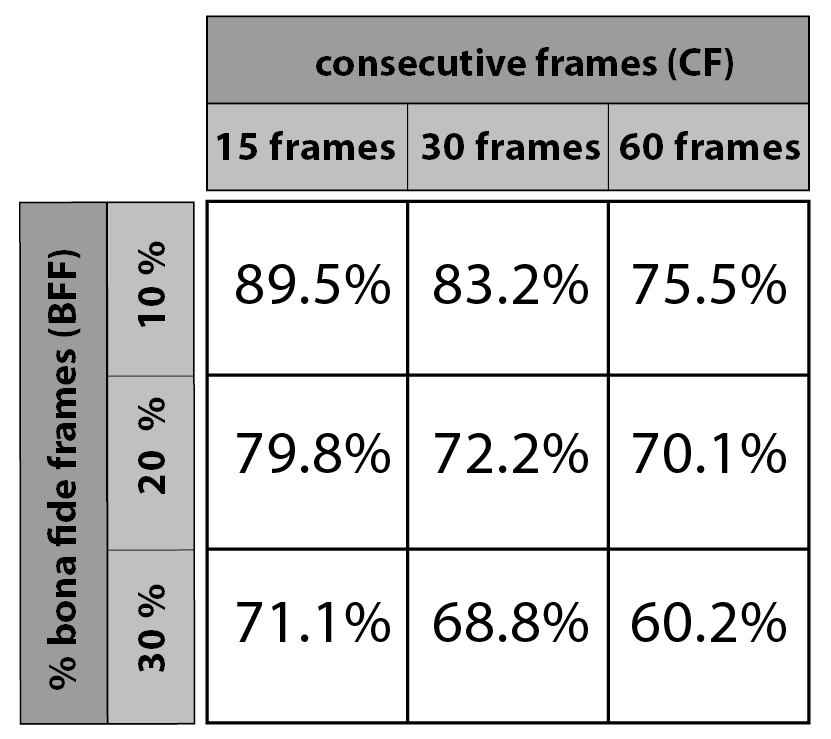
\includegraphics[width=1\linewidth]{ch-sistemasABC/images/ch-onthefly/TRACKING-FRAV-ABC.png}
        \caption{Resultados del módulo \textit{Tracking}.}
        \label{fig:pad-result-REAL-SCENARIO}
    \end{subfigure}
    \caption{Resultados del módulo \GLS{PAD} y del módulo \textit{tracking} con los vídeos base de datos \Gls{FRAV-ABC-OnTheFly}.}
    \label{fig:ranges-APCER-BPCER-RESULT_OnTheFly}
\end{figure}

\begin{table}[t!]
\centering
\begin{tabular}{|c|c|c|c|c|}
\hline
\textbf{Range} & \textbf{PAI} & \textbf{APCER(\%)} & \textbf{BPCER(\%)} & \textbf{D-EER(\%)} \\ \hline 
\multirow{5}{*}{\textbf{Range-1}} &Photo& $0.180$ & $0.112$ & $0.146$ \\ \cline{2-5} 
                                  &Mask & $0.425$ & 0.062 & $0.243$ \\ \cline{2-5} 
                                  & Mask w/o eyes& $0.280$ & $0.152$ & $0.216$ \\ \cline{2-5} 
                                  & Video   & $0.075$ & $0.385$ & $0.422$ \\ \cline{2-5} 
                                  & $3$D Mask & $0.412$ & $0.022$ & $0.217$ \\ \cline{2-5}
                                  & \textbf{All attacks} & $\textbf{0.102}$ & $\textbf{0.086}$ & $\textbf{0.094}$ \\ \hline
\multirow{5}{*}{\textbf{Range-2}} &Photo& $0.033$ & $0.052$ & $0.042$ \\ \cline{2-5} 
                                  &Mask& $0.044$ & $0.085$ & $0.064$ \\ \cline{2-5} 
                                  &Mask w/o eyes& $0.098$ & $0.015$ & $0.056$ \\ \cline{2-5} 
                                  &Video& $0.093$ & $0.102$ & $0.097$ \\ \cline{2-5} 
                                  & $3$D Mask & $0.091$ & $0.013$ & $0.052$ \\ \cline{2-5}
                                  & \textbf{All attacks} & $\textbf{0.026}$ & $\textbf{0.019}$ & $\textbf{0.022}$ \\ \hline
\multirow{5}{*}{\textbf{Range-3}} &Photo & $0.103$ & $0.052$ & $0.077$ \\ \cline{2-5} 
                                  &Mask& $0.345$ & $0.090$ & $0.217$ \\ \cline{2-5} 
                                  &Mask w/o eyes& $0.141$ & $0.285$ & $0.213$ \\ \cline{2-5} 
                                  &Video& $0.258$ & $0.281$ & $0.269$ \\ \cline{2-5} 
                                  &$3$D Mask& $0.587$ & $0.030$ & $0.308$ \\ \cline{2-5}
                                  & \textbf{All attacks} & $\textbf{0.098}$ & $\textbf{0.106}$ & $\textbf{0.102}$ \\ \hline
\end{tabular}
\caption{Resultados del módulo \GLS{PAD} por rango y por tipo de \GLS{PAI} en los vídeos de la base de datos \Gls{FRAV-ABC-OnTheFly}.}
\label{tab:result_PAD_Database}
\end{table}


La Fig. \ref{fig:ranges-APCER-BPCER-RESULT_OnTheFly} (a) muestra los resultados del módulo \GLS{PAD} de forma aislada, con imágenes extraídas de los vídeos de la base de datos \Gls{FRAV-ABC-OnTheFly}. Y Fig. \ref{fig:ranges-APCER-BPCER-RESULT_OnTheFly} (b), presenta los resultados de procesar estos mismos vídeos al completo, con el módulo de \textit{tracking}, es decir, teniendo en cuenta los fallos de detección, además de los ataques de presentación detectados.

\medskip
\textbf{\Gls{FRAV-OnTheFly} anaálisis \gls{OnTheFly}} % Onthefly en lab
\medskip

Cuando se trata de sistemas \GLS{ABC} en los que prevalece la seguridad, resulta apropiado aumentar el porcentaje de \textit{frames bona-fide}. Al menos un $30$\% de \GLS{BFF} es valor que garantiza la seguridad del sistema. Y atendiendo a las pruebas realizadas, un $15$ de \GLS{CF} es una opción fiable para una distancia de $3$ metros. Bajo estos criterios de configuración el sistema alcanza una precisión del $71,1$\%.


\medskip
\textbf{\Gls{FRAV-OnTheFly} análisis estático} % Estatico en lab
\medskip

La Fig. \ref{fig:ranges-APCER-BPCER-RESULT_OnTheFly} (a) presenta los resultados del sistema sin tener en cuenta el \textit{tracking}, sólo el módulo \GLS{PAD}. Para aislar la detección de ataques, se han segmentado todas las caras en los vídeos de test de base de datos \Gls{FRAV-OnTheFly} y se han agrupado estimando el rango al que pertenece la cara detectada. Las imágenes de cada conjunto se ha clasificado con los \GLSpl{SVM} del rango de distancias correspondiente del repositorio de modelos.

Las curvas \GLS{DET} con los errores \GLS{APCER} y \GLS{BPCER} obtenidos en cada rango muestran que el \textit{Rango-2} es el que tiene la menor tasa de error \GLS{D-EER}, lo que indica que la distancia a la que mejor se detectan los errores es una distancia intermedia mayor de $1$ m e inferior a $2$ m. Analizando en detalle las curvas para cada rango, aunque las tasas de error son bajas en los tres, se puede ver que las imágenes que están a más de $2$ m de distancia tienen el peor resultado en el módulo \GLS{PAD}. Esto se debe al tipo de características empleadas para clasificar, al estar basado en texturas (\GLS{LBP}) no son discriminantes cuando las imágenes están demasiado alejadas del dispositivo y la captura es demasiado ruidosas y con artefactos.

La tabla \ref{tab:result_PAD_Database} muestra las tasas \GLS{APCER} y \GLS{BPCER} y el \GLS{D-EER} de cada uno de los clasificadores del depósito para un rango dado y con un \GLS{PAI} determinado. Se confirma que las tasas de error en la detección de ataque son más bajas en el rango $2$ para todos los ataques. Y además, se puede observar que el ataque más fácil de detectar es el ataque con foto. Mientras que los ataques con vídeo y con máscaras $3$D son los más difícilmente detectables.
\medskip

\subsection{Resultados del escenario de la frontera real}%% EN FRONTERA REAL

\begin{figure}[t!]
    \centering
    \begin{subfigure}{.45\textwidth}
        \centering
        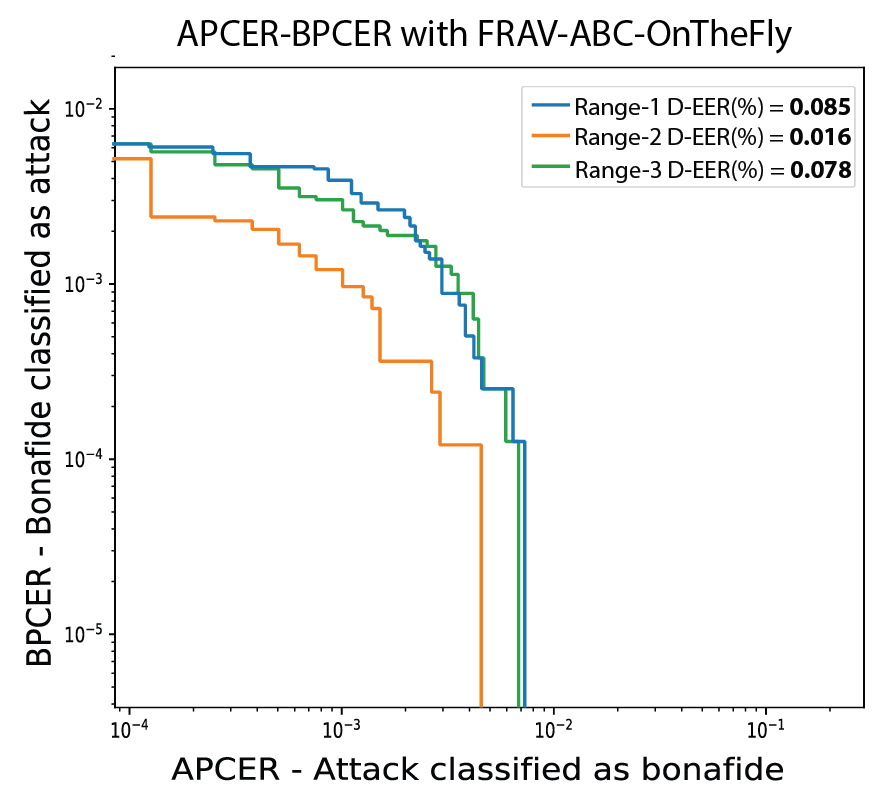
\includegraphics[width=1\linewidth]{ch-sistemasABC/images/ch-onthefly/APCER-BPCER-WITH-FRAV-ABC_b.png}
        \caption{Resultados del modulo \emph{PAD} por rangos}
        \label{fig:result_matrix_database}
    \end{subfigure}
    \begin{subfigure}{.45\textwidth}
        \centering
        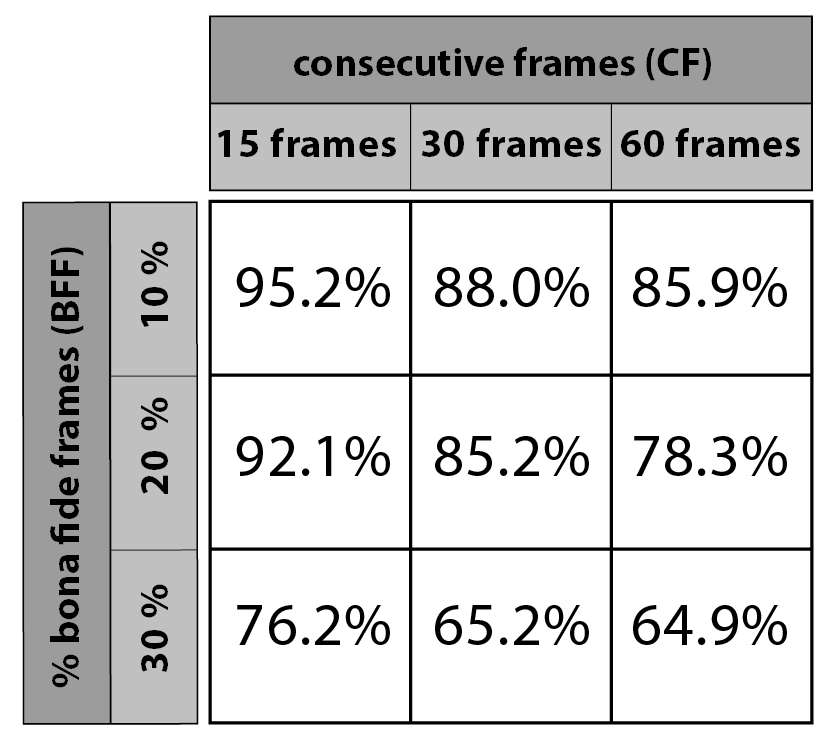
\includegraphics[width=1\linewidth]{ch-sistemasABC/images/ch-onthefly/TRACKING-DEVICE.png}
        \caption{Precisión del modulo \emph{Tracking}}
        \label{fig:result_matrix_real}
    \end{subfigure}
    \caption{Resultados del módulo \GLS{PAD} y del módulo \textit{tracking} con los vídeos base de datos \Gls{FRAV-ABC-OnTheFly}.}
    \label{fig:APCER-BPCER-RESULT-ABC-OnTheFly}
\end{figure}


\begin{table}[t!]
\centering
\begin{tabular}{|c|c|c|c|c|}
\hline
\textbf{Range} & \textbf{PAI} & \textbf{APCER(\%)} & \textbf{BPCER(\%)} & \textbf{D-EER(\%)} \\ \hline 
\multirow{5}{*}{\textbf{Range-1}} &Photo& $0.144$ & $0.100$ & $0.123$ \\ \cline{2-5} 
                                  &Mask& $0.416$ & $0.050$ & $0.234$ \\ \cline{2-5} 
                                  &Mask w/o eyes& $0.252$ & $0.123$ & $0.188$ \\ \cline{2-5} 
                                  &Video& $0.058$ & $0.382$ & $0.220$ \\ \cline{2-5} 
                                  &$3$D Mask& $0.403$ & $0.000$ & $0.202$ \\ \cline{2-5}
                                  &$\textbf{all attacks}$&$\textbf{0.092}$ &$\textbf{0.070}$ &$\textbf{0.085}$ \\ \hline
\multirow{5}{*}{\textbf{Range-2}} &Photo& $0.024$ & $0.037$ & $0.031$ \\ \cline{2-5} 
                                  &Mask& $0.037$ & $0.063$ & $0.050$ \\ \cline{2-5} 
                                  &Mask w/o eyes & $0.063$ & $0.024$ & $0.043$ \\ \cline{2-5} 
                                  &Video& $0.116$ & $0.074$ & $0.095$ \\ \cline{2-5} 
                                  &$3$D Mask& $0.050$ & $0.000$ & $0.025$ \\ \cline{2-5}
                                  &$\textbf{all attacks}$ & $\textbf{0.018}$ & $\textbf{0.020}$ & $\textbf{0.016}$ \\ \hline
\multirow{5}{*}{\textbf{Range-3}} &Photo & $0.096$ & $0.037$ & $0.067$ \\ \cline{2-5} 
                                  &Mask& $0.340$ & $0.100$ & $0.221$ \\ \cline{2-5} 
                                  &Mask w/o eyes& $0.126$ & $0.296$ & $0.211$ \\ \cline{2-5} 
                                  &Video& $0.290$ & $0.234$ & $0.262$ \\ \cline{2-5} 
                                  &$3$D Mask & $1.209$ & $0.000$ & $0.605$ \\ \cline{2-5}
                                  &$\textbf{all attacks}$ & $\textbf{0.080}$ & $\textbf{0.078}$ & $\textbf{0.078}$ \\ \hline
\end{tabular}
\caption{Resultados del módulo \GLS{PAD} por rango y por tipo de \GLS{PAI} en los vídeos de la base de datos \Gls{FRAV-ABC-OnTheFly}.}
\label{tab:result_PAD_Real}
\end{table}

\medskip
\textbf{\Gls{FRAV-ABC-OnTheFly} análisis \gls{OnTheFly}} % Onthefly en real
\medskip

La Fig. \ref{fig:APCER-BPCER-RESULT-ABC-OnTheFly} presenta los resultados del sistema con los vídeos de la base de datos \Gls{FRAV-ABC-OnTheFly}, que se obtuvo en el escenario real de cruce de fronteras. Aunque algunas condiciones como la iluminación o el fondo de la captura, no están tan controladas, los resultados son similares a los obtenidos en la base de datos \Gls{FRAV-OnTheFly}.

Aunque se logran valores de precisión más altos considerando un porcentaje menor de \textit{frames} detectados como \textit{\gls{bona-fide}} (\GLS{BFF}), es conveniente que el sistema sea más restrictivo, ya que los sistemas \GLS{ABC} requieren un alto nivel de seguridad y una alerta falsa con un viajero \textit{\gls{bona-fide}}) siempre puede ser atendida manualmente por los agentes de seguridad. Al igual que con la base de datos \Gls{FRAV-OnTheFly}, un $30$\% de \GLS{BFF} de un \textit{tracking} de al menos $15$ \GLS{CF}, es una buena elección y garantiza una precisión del $76,2$\%. 

\medskip
\textbf{\Gls{FRAV-ABC-OnTheFly} análisis Estático} % Estatico en real
\medskip

La Fig. \ref{fig:APCER-BPCER-RESULT-ABC-OnTheFly} (a) muestra la \textit{curva \GLS{DET} con las tasas de error de \GLS{APCER} y \GLS{BPCER} por rango en el escenario real}. Aunque las tasas de error son bajas en los tres rangos, el rango con el menor error de detección es el \textit{Rango-2}. La pérdida de calidad de las imágenes (capturadas demasiado lejos o demasiado cerca) penaliza el rendimiento del módulo \GLS{PAD}. Al igual que en los datos del laboratorio (Tabla \ref{tab:result_PAD_Database}), esto también se desprende claramente de los resultados presentados en la Tabla \ref{tab:result_PAD_Real} donde se detalla el rendimiento de cada clasificador en el depósito de modelos con las caras segmentadas en el entorno real. 
\medskip

Lo experimentos muestran la viabilidad del sistema \gls{FlyPAD}. El sistema alcanza valores de precisión muy similares a otros sistemas que funcionan en escenarios reales con captura estática \cite{komulainen2019review}. Se puede establecer que la propuesta funciona con éxito tanto en situaciones estáticas como dinámicas. Esta cuestión lleva a pensar en una futura implantación del sistema en cruces fronterizo, incrementado el flujo de viajeros, reduciendo los tiempos de cruce  y con procedimientos biométricos menos intrusivos.

%%%%%%%%%%%%%% CONCLUSIONES %%%%%%%%
\section{Conclusiones}\label{sec:ConclusuionesFlayPAD}

En este capitulo se ha presentado \gls{FlyPAD}, un \GLS{PAD} para sistemas \GLS{ABC} capaz de llevar a cabo la detección de ataques de presentación dinámicamente mientras los viajeros cruzan la frontera. Cubre cinco tipos diferentes de ataque relacionados con la biometría facial: fotos impresas, máscaras de papel, máscaras de papel sin ojos, vídeos en pantalla y máscaras $3$D. 

La arquitectura de sistema consta de cuatro módulos: el principal es el módulo de \textit{tracking} que genera un \textit{token} con la información del viajero. Está apoyado por el módulo de detección, el módulo de verificación y el módulo \GLS{PAD}. Este último utiliza diferentes modelos de aprendizaje automático previamente entrenados para tres distancias de adquisición diferentes para realizar la detección de ataques de presentación.

Para probar la propuesta se han llevado a cabo varios experimentos en un entorno controlado y también en un entorno real. Los resultados obtenidos permiten concluir que \gls{FlyPAD} es capaz de detectar dinámicamente, posibles ataques de presentación. La precisión de esta detección detección puede configurarse atendiendo a un umbral para reducir el número de falsos positivos, aumentando la robustez del sistema en un entorno real. En cuanto a las tres distancias de adquisición, los peores resultados fueron para el Rango-3, el más cercano al dispositivo de captura. En este caso, las imágenes tienen una mayor resolución y producen un mayor \GLS{D-EER} en comparación con los otros intervalos. Esto está relacionado con las texturas calculadas en el algoritmo \GLS{LBP}, que pueden variar demasiado para dicha resolución.

Como conclusión general, los resultados obtenidos en el entorno real son mejores que los obtenidos en el laboratorio, probablemente porque las pruebas de laboratorio han sido más exhaustivas y también porque se disponía de más muestras. Además, se ha detectado que ciertos ataques pierden su eficacia directamente en el enfoque \gls{OnTheFly}, porque a ciertas distancias no se detectan los \gls{PAI} como los rasgos biométricos de los individuos. Este problema inhabilita estas situaciones como posibles ataques.

El sistema \gls{FlyPAD} es un prototipo funcional que ha sido puesto a prueba con éxito. Sin embargo, puede resultar interesante validar algunas directrices futuras que podrían mejorar sus capacidades. Por ejemplo, se pueden incluir ataques con nuevos \GLS{PAI} como máscaras de silicona ( \cite{agarwal2017swapped}; \cite{manjani2017detecting}) y también implementar otros algoritmos en el módulo \GLS{PAD} que consideren la información temporal del desplazamiento del viajero y las características espaciales, como redes \textit{Long short-term memory} (\GLS{LSTM}) ( \cite{xu2015learning}) podrían ser interesantes en este momento.


% En el caso del \Gls{FlyPAD}, ha sido probado preliminarmente en un laboratorio que simula un cruce de frontera. Luego, se ha incluido en un sistema \GLS{ABC} con puertas electrónicas en un escenario fronterizo real. Ambas perspectivas han demostrado la viabilidad del prototipo. Sin embargo, este marco tiene como objetivo principal la \GLS{PAD} dinámica. Esto hace que el sistema se adapte mejor a la topología Segregada de Dos Pasos, ya que el sistema realiza una verificación facial después de haber registrado previamente la información del viajero. También es interesante mencionar que la detección de documentos de viaje manipulados está fuera del alcance del \Gls{FlyPAD}.
